\scanpage{76}
\mspage{37}
9) \uline{The groupoid structure of the} \inserted{\uline{moduli spaces of}} \uline{Teichmuller} \uline{moduli} (the MDT-structure) : transcendental case, generization morphisms.

We now work with the $M^{\mathrm{an}}_{g,\nu}$, $\widehat M^{\mathrm{an}}_{g,\nu}$ and so on -- and so as not to drag along the superscripts ``an'' (for ``analytic''), we drop them.

Let us consider for every MD-graph $\underline G$, the modular (analytic) multiplicity $M_{\underline G}$, and its fundamental groupoid, which I denote by $\Pi M_{\underline G}$. It is a \inserted{``large''} category, in what follows we shall see how to replace \unsure{it|it} \inserted{\unsure{canonical\textsuperscript{ly}}} by a \deleted{category} \inserted{groupoid} whose set of objects is finite. In our constructions, it is indeed permissible to replace a groupoid such as $\Pi M_{\begin{tikzpicture}[baseline=(g.base),x=1ex,y=1ex]
\node[inner sep=0pt,outer sep=0pt] (g) at (0,0) {$\scriptstyle\underline G$};
\node[inner sep=0pt,outer sep=0pt,anchor=south] at (-0.08,0.25) {$\unsure{\begin{tikzpicture}[x=0.65ex,y=0.65ex,baseline=0pt]
\draw[line width=0.28pt] (0,0) -- (-0.11,1.18);
\draw[line width=0.28pt] (-0.04,0.59) -- (0.24,0.92);
\end{tikzpicture}}$};
\end{tikzpicture}}$ by an equivalent groupoid, provided that \deleted{the equivalence} \inserted{in the latter} $\underset{\unsure{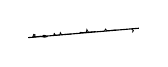
\begin{tikzpicture}[x=1em,y=1em,baseline=0pt]
\draw[line width=0.4pt] (0,0) -- (4.0,0.34);
\draw[line width=0.3pt] (0.16,0.015) -- (0.20,0.12) -- (0.25,0.10) -- (0.21,0.02)
 -- (0.35,0.04) .. controls (0.48,0.10) and (0.53,-0.04) .. (0.68,0.035)
 .. controls (0.59,0.12) and (0.51,0.08) .. (0.50,0.045);
\draw[line width=0.3pt] (0.92,0.08) -- (0.94,0.15) -- (0.99,0.08)
 -- (1.14,0.10) -- (1.16,0.18) -- (1.20,0.11) -- (1.56,0.13);
\draw[line width=0.3pt] (1.86,0.16) .. controls (1.88,0.26) and (1.90,0.14) .. (1.98,0.18)
 -- (2.10,0.20) -- (2.12,0.29) -- (2.17,0.20) -- (2.44,0.22);
\draw[line width=0.3pt] (2.76,0.24) -- (2.79,0.31) -- (2.85,0.25) -- (3.19,0.28);
\draw[line width=0.3pt] (3.73,0.32) -- (3.80,0.25) -- (3.76,0.19);
\end{tikzpicture}}}{\text{the group}}$
\[
(94)\qquad \Gamma_{\underline G}=\operatorname{Aut}\underline G
\]
acts, and that the equivalence commutes with the \unsure{action} of this group.

Let us note already that $\Pi M_{\underline G}$ is a groupoid
\margin{75}
